\documentclass{beamer}
%
% Choose how your presentation looks.
%
% For more themes, color themes and font themes, see:
% http://deic.uab.es/~iblanes/beamer_gallery/index_by_theme.html
%
\mode<presentation>
{
  \usetheme{default}      % or try Darmstadt, Madrid, Warsaw, ...
  \usecolortheme{default} % or try albatross, beaver, crane, ...
  \usefonttheme{default}  % or try serif, structurebold, ...
  \setbeamertemplate{navigation symbols}{}
  \setbeamertemplate{caption}[numbered]
} 

\usepackage[english]{babel}
\usepackage[utf8x]{inputenc}
\usepackage{xcolor}
\usepackage{makecell}

\title{Alkylresorcinol (AR) Can Not Indicate Whole Grain Barley Intake}

\author{Tu Hu \newline \tiny{ Supervisor: Gözde \& Lars}}
\institute{University of Copenhagen}
\date{8th, Feb, 2019}
%% Hi, Henrik and Gözde. Thank you for coming to my exam. I'll present my project to you.
%% The topic is Discovering Barley Intake Biomarkers in Urine by UPLC-MS Based Untargeted Metabolomics. My supervisor is Gözde. 


\begin{document}

\begin{frame}
  \titlepage

  \tiny{@GitHub/tuhulab/bfi-wholegrain/presentation}
\end{frame}

%%
\begin{frame}{Outline}
  \tableofcontents
\end{frame}
%% This is the outline of my presentation.
%% First, I'll first introduce the Background (how the intervention was performed and how the samples were collected)
%% Then, I'll present why we research on barley, why we need to research barley's intake biomarker? What is the societal and scientific importance? and the general workflow for untargeted metabolomics methods for barley intake biomarkers discovery.
%% Then, I'll shortly introduce materials & methods. just some key points.
%% My presentation today will emphasize on results and comclusions.
%% In the end, I'll present perspectives, what i'm going to do in next step.

\section{Study Design}
 \begin{frame}{Study Design}
 \begin{figure}[h]
    \centering
    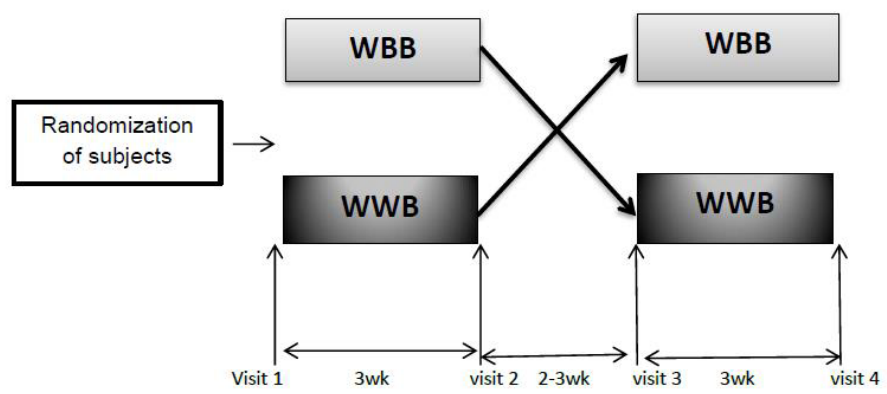
\includegraphics[scale=0.3]{images/studes.PNG}
    \caption{Schema of Study Design (WBB=whole barley bread; WWB=whole wheat bread)}
        \label{fig:studes}
\end{figure}
{\footnotesize
\begin{itemize}
\item randomized cross-over intervention design. \textbf{In wash-out period, subjects did not have any dietary restrictions}
\item 2 bread rolls/day during intervention period
\item 14 healthy volunteers (6 men, 8 women)
\item fasting plasma \& 24-h pooled urine samples
\item Conclusion: No significant changes of CVD risk factors and other health statue factors (before \& after intervention; after barley \& wheat)
\end{itemize}}
 \end{frame}
 %% So, first, background. This study was actually based on a previous master thesis in 2016. A randomized cross-over intervention study was designed. During intervention period, the volunteers consumed 2 bread rolls each day.
 %% The conclusion was there's no significant changes of these factors (before & after intervention : the change is not significant) (barley intervention and wheat intervention no significant changes)
 

% P1
\section{Alkylresorcinols (AR) in Literature}
%%
\begin{frame}{Alkylresorcinols: biomarkers of whole grain cereal intake}
\textbf{Current status}
\begin{itemize}
	\item Widely reported and validated biomarker for whole grain cereals (Table)
	\item Detected both in urine and plasma
\end{itemize}

\textbf{Limitations}
\begin{itemize}
	\item Taking account of all whole grain cereals. 
	\item Not specific to individual grain type (wheat, rye, oats, barley...)
	\item No barley biomarkers reported
\end{itemize}
\end{frame}

%%

\begin{frame}{Alkylresorcinols (updated until Nov, 2018)}
\begin{figure}[h]
    \centering
    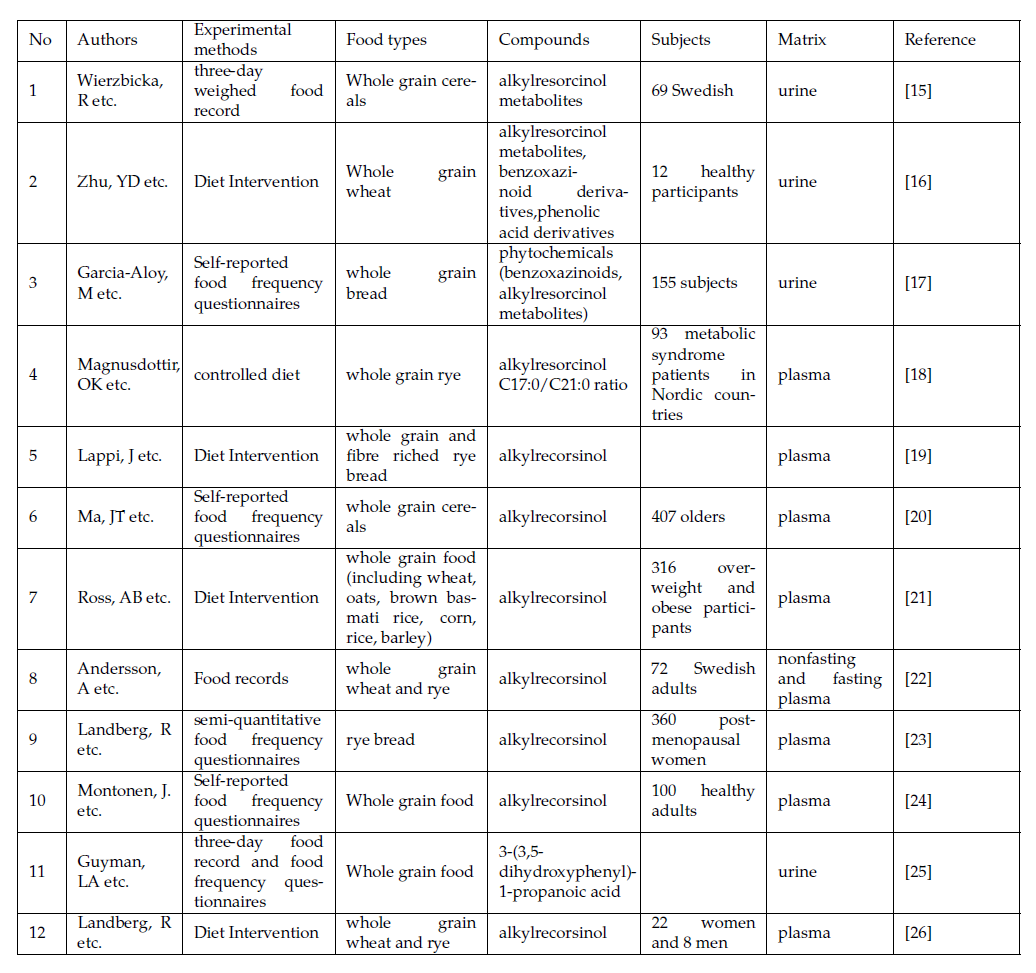
\includegraphics[scale=0.32]{images/alkylresorcinols.png}
\end{figure}
\end{frame}


\section{AR in Barley Dataset}
\begin{frame}{AR in Barley Dataset: serum}

{\tiny
\begin{tabular}{|c|c|c|c|c|c|c|}
	\hline 
	& Formula & Reference RT & Reference MZ & Annotation & Detected RT & Detected MZ \\ 
	\hline 
	\makecell{AR(C21:0) \\ glucuronide} & C33H56O8 & 5.03 & 579.389 & [M-H]- & 5.0222 & 579.3902 \\ 
	\hline 
	\makecell{AR(C21:1) \\ glucuronide} & C33H54O8 & 4.92 & 577.375 & [M-H]- & 4.9199 & 577.3736 \\ 
	\hline 
	\makecell{AR(C19:0) \\ glucuronide} & C31H52O8 & 4.92 & 551.360 & [M-H]- & 4.9143 & 551.3579 \\ 
	\hline 
\end{tabular} }
	
	\begin{columns}
	\column{0.5\textwidth}
	\begin{figure}[h]
		\centering
		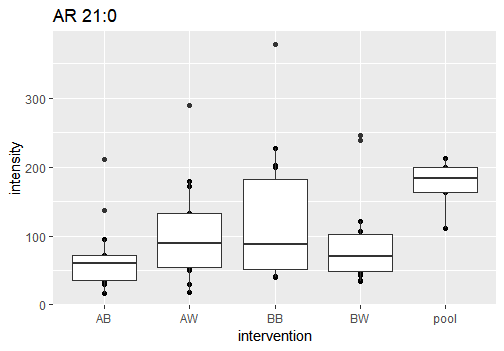
\includegraphics[scale=0.4]{images/ar210.PNG}
	\end{figure}

	\column{0.5\textwidth}
		\begin{figure}[h]
		\centering
		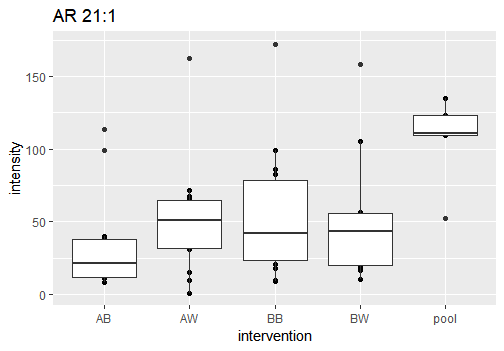
\includegraphics[scale=0.4]{images/ar211.PNG}
	\end{figure}
	\end{columns}
\tiny
AB=After Barley \\
AW=After Wheat \\
BB=Before Barley\\
BW=Before Wheat \\
\end{frame}

\begin{frame}{AR in Barley Dataset: serum}

{\tiny
	\begin{tabular}{|c|c|c|c|c|c|c|}
		\hline 
		& Formula & Reference RT & Reference MZ & Annotation & Detected RT & Detected MZ \\ 
		\hline 
		\makecell{AR(C21:0) \\ glucuronide} & C33H56O8 & 5.03 & 579.389 & [M-H]- & 5.0222 & 579.3902 \\ 
		\hline 
		\makecell{AR(C21:1) \\ glucuronide} & C33H54O8 & 4.92 & 577.375 & [M-H]- & 4.9199 & 577.3736 \\ 
		\hline 
		\makecell{AR(C19:0) \\ glucuronide} & C31H52O8 & 4.92 & 551.360 & [M-H]- & 4.9143 & 551.3579 \\ 
		\hline 
\end{tabular} }

\begin{columns}
	\column{0.5\textwidth}
	\begin{figure}[h]
		\centering
		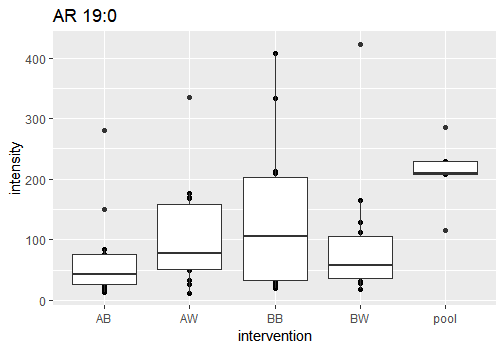
\includegraphics[scale=0.4]{images/ar190.PNG}
	\end{figure}

\end{columns}

\end{frame}

\begin{frame}{AR in Barley Dataset: urine}
\centering
{
 \tiny
\begin{tabular}{|c|c|c|c|c|c|c|}
	\hline 
	Molecular & Formula & Reference RT & Reference MZ \\ 
	\hline 
	\makecell{3,5 DHPPA \\ glucuronide} & C15H18O10 & 1.98 & 357.09\\ 
	\hline 
	\makecell{3,5 DHBA \\ glucuronide} & C33H14O10 & 0.93 & 329.051\\ 
	\hline 
	\makecell{3,5 DHPPA} & C9H10O4 & 2.66 & 181.041\\
	\hline
	\makecell{3,5DHBA} & C7H6O4 & 1.94 & 153.018 \\
	\hline
	 
\end{tabular}}

\begin{columns}
	\column{0.5\textwidth}
	\begin{figure}[h]
				\centering
		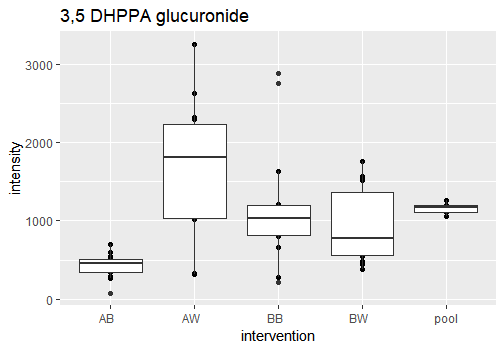
\includegraphics[scale=0.4]{images/35dhppag.PNG}
	\end{figure}
	
	\column{0.5\textwidth}
		\begin{figure}[h]
		\centering
		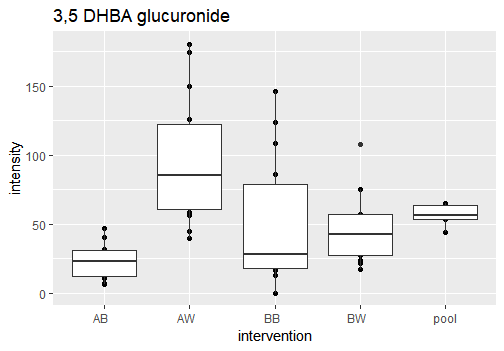
\includegraphics[scale=0.4]{images/35dhbag.PNG}
	\end{figure}
\end{columns}

\end{frame}

\begin{frame}{AR in Barley Dataset: urine}
\centering
{
	\tiny
	\begin{tabular}{|c|c|c|c|c|c|c|}
		\hline 
		Molecular & Formula & Reference RT & Reference MZ \\ 
		\hline 
		\makecell{3,5 DHPPA \\ glucuronide} & C15H18O10 & 1.98 & 357.09\\ 
		\hline 
		\makecell{3,5 DHBA \\ glucuronide} & C33H14O10 & 0.93 & 329.051\\ 
		\hline 
		\makecell{3,5 DHPPA} & C9H10O4 & 2.66 & 181.041\\
		\hline
		\makecell{3,5DHBA} & C7H6O4 & 1.94 & 153.018 \\
		\hline
		
\end{tabular}}

\begin{columns}
	\column{0.5\textwidth}
	\begin{figure}[h]
		\centering
		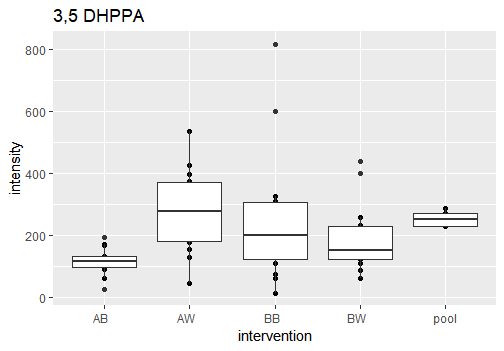
\includegraphics[scale=0.4]{images/35dhppa.PNG}
	\end{figure}
	
	\column{0.5\textwidth}
	\begin{figure}[h]
		\centering
		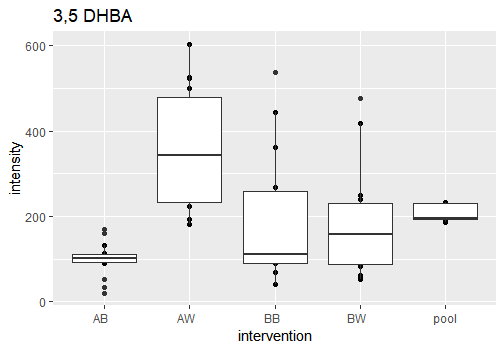
\includegraphics[scale=0.4]{images/35dhba.PNG}
	\end{figure}
\end{columns}

\end{frame}

\section{Conclusion \& Feedback}
\begin{frame}{Conclusion \& Feedback}
\begin{itemize}
	\item Subjects regularly consume whole grain food. But exposure amount varied individually.
	\begin{itemize}
		\item Background value in 'BB', 'BW' groups	
		\item High deviation in 'BB', 'BW' groups
	\end{itemize}

	\item AR metabolites in serum can indicate long-term (cumulative) whole grain food exposure.
	\item AR metabolites in urine can indicate short-term whole grain food exposure.
	\item However, AR can not indicate whole grain barley intake
		\begin{itemize}
		\item AR conc. decreased in 'AB' group
		\end{itemize}
	
	\item Questions
	\begin{itemize}
		\item Safer conclusion?
		\item Better statistics or visualization method to reveal conclusions?
		\item Compare AR conc. in barley \& wheat?
	\end{itemize}

	
	
\end{itemize}

\end{frame}
\end{document}
